\chapter{Introducción}
\chapterquote{Avanza rapido el tema de las tortugas}{D. H. Zanette}

\section{ C. \textit{chilencis} }
\label{S:opciones-que-acepta}

La mayoría de las especies animales son capaces de realizar complejos patrones de movimientos que generalmente dependen del ambiente, factores intrínsecos de los individuos y las interacciones entre ellos (\cite{morales2005adaptive}, \cite{morales2010building} y \cite{nathan2008emerging}). La complejidad de estos movimientos están manifestados en sus trayectorias. Para el caso de las tortugas estas trayectorias dependen fuertemente de la vegetación en la zona de estudio y la época del año (caso que busquen reproducirse, depositar sus huevos, etc.).


Nuestra especie de interés es la tortuga $Chelonoidis$ $chilensis$. Se distribuye desde el Gran Chaco hasta el norte de la Patagonia, como se muestra en la Fig.~\ref{fig:distribuciondeEspecie} (\cite{chebez2008se}). Esta especie está incluida en el Appendix  de la \textit{Convention on International Trade in Endangered Species of Wild Fauna and Flora (CITES)} y fue categorizada como \textit{vulnerable} a nivel nacional \cite{prado2012categorizacion} e internacional por la \textit{International Union for Conservation of Nature (IUCN)}.
Los principales factores que llevaron a esta situación son la reducción, modificación y destrucción de su hábitat, debido a la expansión de la frontera agropecuaria, y su comercialización, siendo la especie nativa de reptiles más ilegalmente traficada en el mercado de mascotas en Argentina (\cite{prado2012categorizacion}). Además, la amenaza a esta especie se ve aumentada con la introducción de especies depredadoras exóticas como el Jabalí (\textit{Sus scrofa}) (\cite{kubisch2014chelonoidis}). En este trabajo estudiaremos una población de tortugas en en el límite sur de su distribución geográfica, a 20 km al norte de San Antonio Oeste, provincia de Río Negro.  \\
    
Las tortugas son animales  herbívoros que se alimentan con tallos y frutos de cactus (\textit{Opuntia sulphurea, Cereus aethiops, Perocactus tuberosus}), gramíneas (\textit{Chloris castilloniana, Trhichloris crinita}), herbáceas (\textit{Alternanthera pugens, Sphaeralcea miniata, S. mendocina, Portulaca grandiflora}) y vainas de leguminosas (\cite{zacarias2016biologia}).
    
    
    
\begin{figure}[h]
    \begin{center}
        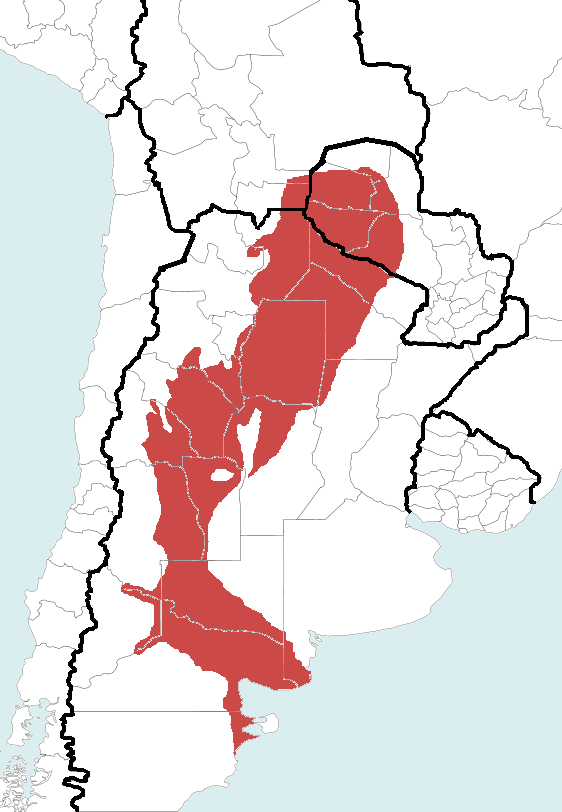
\includegraphics[width=\imsize]{figs/Chap1/Chelonoidis_chilensis_geographic_range.png}
        \caption{Distribución geográfica de la especie de tortuga \textit{Chelonoidis chilensis} \label{fig:distribuciondeEspecie}.}
        
        \end{center}
\end{figure}
Esta especie presenta un dimorfismo sexual cuando son adultos. Los machos son notablemente más chicos que las hembras. El período de actividad en la distribución más sur de la especie es el más corto, ya que bruman (parecido a hibernar) por aproximadamente cinco meses. Sus períodos de actividad comienzan en el mes de septiembre y, desde noviembre a diciembre, es cuando el apareamiento es mayormente observado. Entre enero y marzo es cuando las hembras pasan una gran parte del tiempo buscando un lugar adecuado para enterrar sus huevos \cite{Erika}. Todavía falta mucho por aprender acerca de la biología de la población de C. \textit{chilencis} presente en Argentina.
 
Motivados por la falta de información, el objetivo de este estudio es caracterizar el movimiento de las tortugas en una de las poblaciones en el límite sur de su distribución geográfica. Aprender acerca del movimiento de los individuos es fundamental para entender su rol ecológico en el ecosistema y para diseñar políticas de conservación de la especie y su hábitat.


\section{Metodologias}

Se combinaron diferentes técnicas para estudiar las trayectorias de las tortugas. En este trabajo se caracterizaron las técnicas utilizadas por el grupo de investigación (Física Estadística e Interdisciplinaria) para monitorear las trayectorias de las tortugas en distintas campañas de medición entre enero de 2020 y abril del 2022.
 
En primer lugar se utilizó una técnica de radiotelemetría para localizar la posición de las tortugas, se recibía una señal, a través de un sistema antena-receptor, de un radio transmisor localizado en el caparazón de las tortugas. La segunda técnica de medición consistió en utilizar una unidad de navegación construída en el Centro Atómico, para registrar señales de GPS, sensores inerciales y de temperatura. Sobre el año 2022 se adopto una tercera tecnica, utilizando una unidad de navegación comercial (i-gotU GT120) que toma datos de GPS y hora. En las siguientes subsecciones se proveerán más detalles de ambas metodologías. 
 
\subsection{Radiotelemetría}
Las técnicas de radiotelemetría permiten localizar individuos mediante un sistema de transmisor-receptor-antena. Se utilizaron transmisores Holohil (Grand HOLOHIL Systems Ltd. RI-2B) pegados a los caparazones de las tortugas mediante cinta adhesiva. Estos transmisores emiten un pulso a una determinada frecuencia ($\approx$150 MHz) cada dos segundos. Estos pulsos eran detectados por un sistema de recepción, que consiste en una antena Yagi-Uda conectada a un receptor ATS R410 (Advanced Telemetry Systems,Inc). Esta técnica permite con gran precisión localizar el transmisor y, usando un GPS portátil (Garmin eTrex
x20), determinar la ubicación.
 
A pesar de ser muy precisa espacialmente, esta técnica no posee una buena resolución temporal, necesaria para reconstruir trayectorias confiables. En primer lugar, es necesario seguir constantemente al individuo para tener una mejor resolución temporal. En segundo lugar, el investigador debe acercarse a una distancia considerable de la tortuga para tomar su posición con el GPS. Esto puede alterar el comportamiento de la tortuga y su trayectoria. En la siguiente sección se describe la unidad de navegación, que ofrece una alta resolución temporal en las trayectorias sin perturbar al comportamiento animal.
 
\subsection{Unidad de navegación}
Se desarrolló en el departamento de Ingeniería del Centro Atómico  una unidad de bajo presupuesto para monitorear individuos en su hábitat natural (de ahora en más llamado tortugómetro), que consiste de un receptor GPS, sensores inerciales (acelerómetro y giróscopo) y un sensor de temperatura (Fig.~\ref{fig:tortugometro}). El mismo está alimentado por una batería recargable que le da una autonomía de aproximadamente 15 horas considerando una adquisición del GPS de un punto cada 5-10 minutos. El peso del tortugómetro es de 45 g representando el 3\% del peso de una tortuga de tamaño medio, lo que es aceptable para no disturbar el movimiento del animal. Los datos del receptor de GPS y los sensores inerciales son guardados en una memoria micro-SD. Al final de cada día de monitoreo se descargaron los datos de la memoria y se cargaron las baterías.
 
En este trabajo, se utilizaron datos obtenidos por campañas realizadas por el grupo de investigación. Contaron con 8 de estas unidades en correcto funcionamiento para monitorear las tortugas en cada día de campaña.
\begin{figure}[h]
    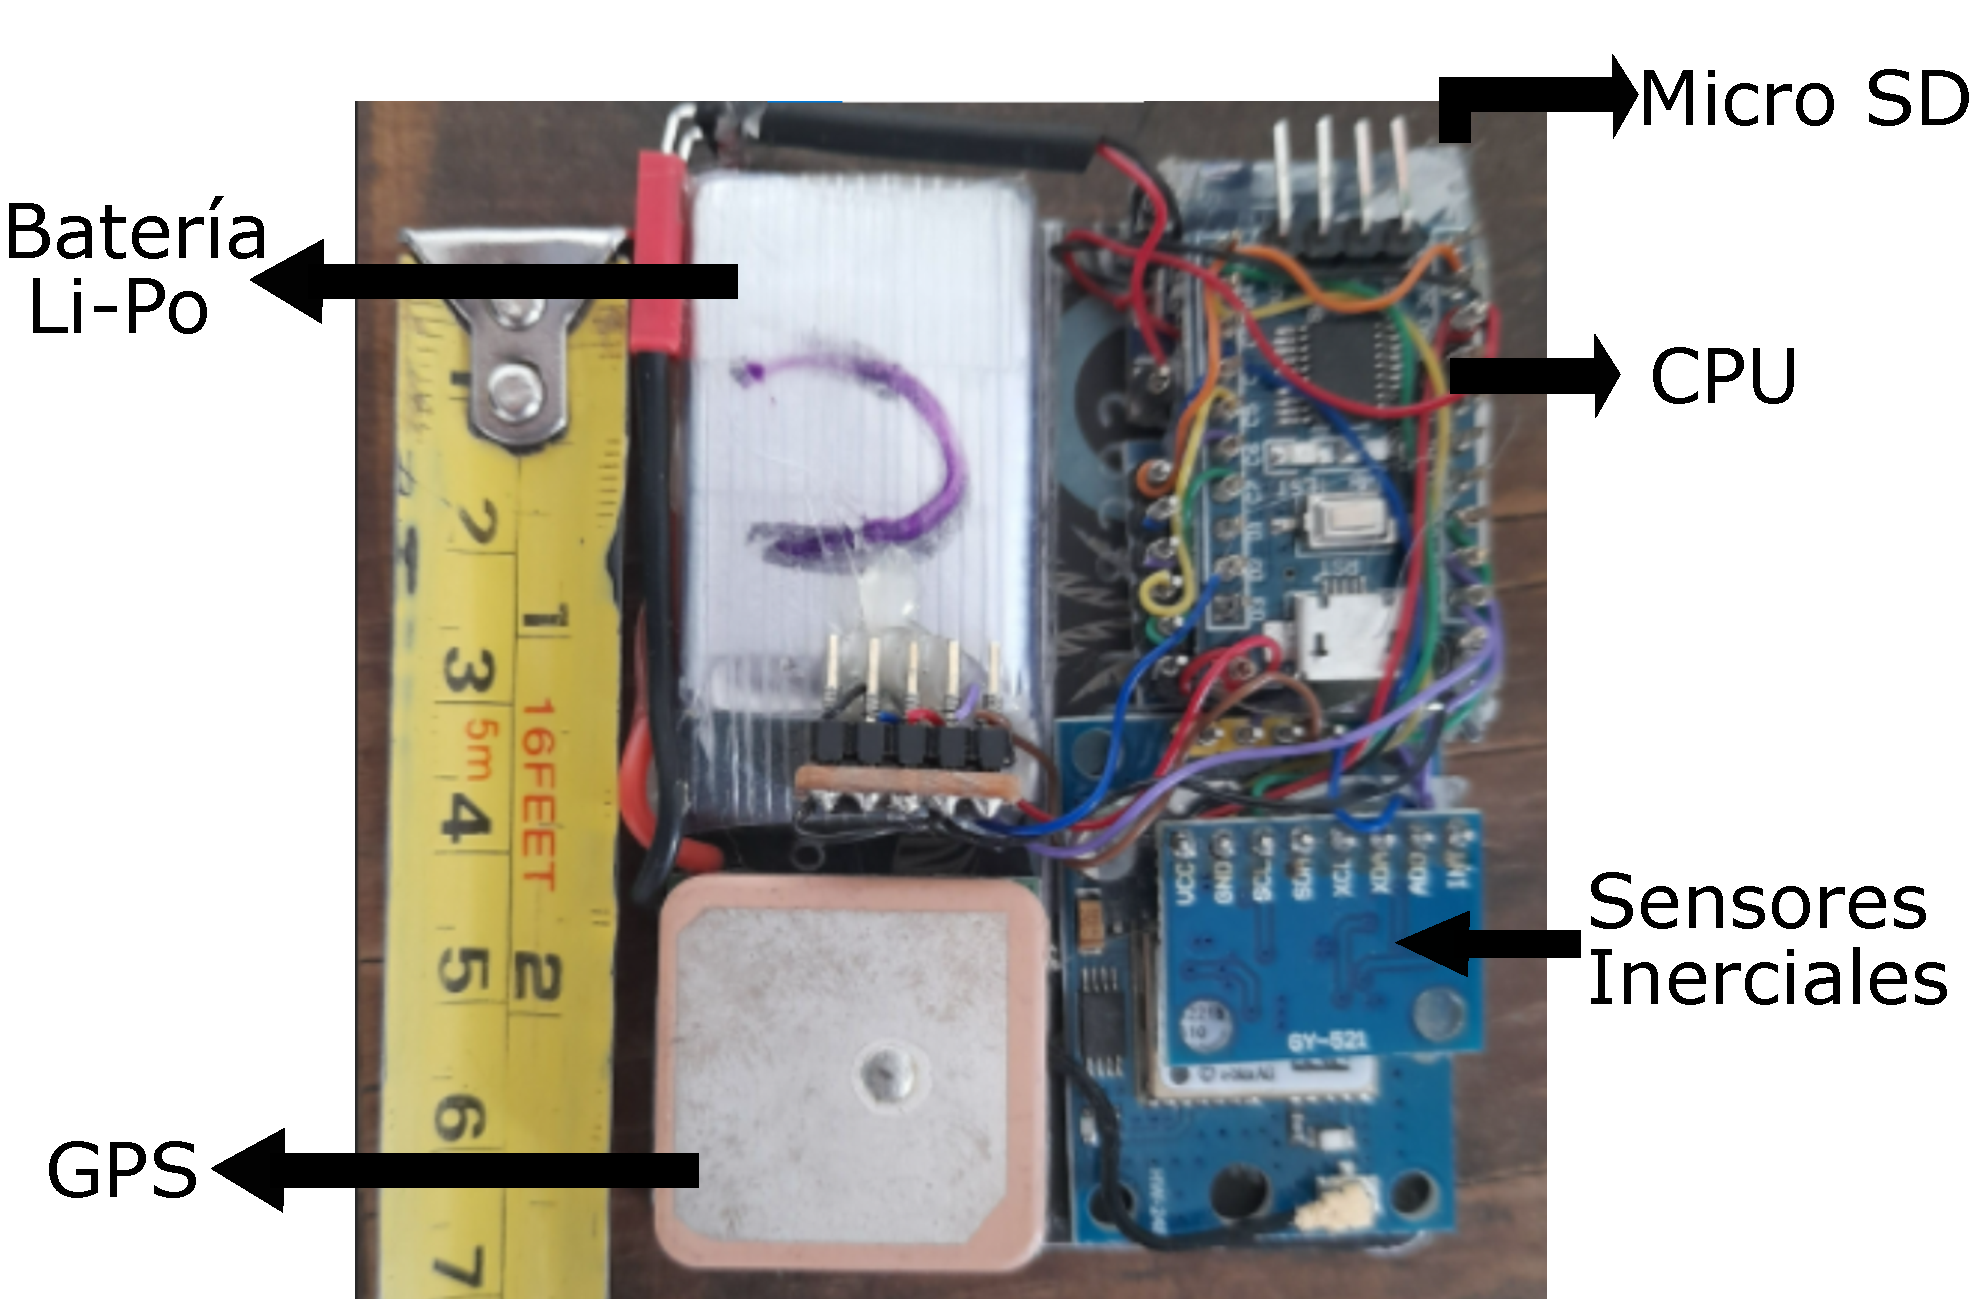
\includegraphics[width=\imsize]{figs/Chap1/tortugometro.pdf}  
    \caption{Unidad de navegación (tortugómetro) para monitorear individuos. Consiste de un GPS, sensores inerciales (giróscopo y acelerómetro) y de temperatura, todos conectados a una unidad de control y procesamiento. Pesa menos de 45g. Las posiciones del GPS son adquiridas cada 10 minutos y se almacenan en la tarjeta micro SD extraíble. }
    \label{fig:tortugometro}
\end{figure}

\subsection{i-gotU}


%%% Local Variables: 
%%% mode: latex
%%% TeX-master: "template"
%%% End: 
